
%\documentclass[smaller,handout]{beamer}
\def\bmode{0} % Mode 0 for presentation, mode 1 for a handout with notes, mode 2 fo% r handout without notes
\if 0\bmode
\documentclass[smaller]{beamer}
\else \if 1\bmode
\immediate\write18{pdflatex -jobname=\jobname-Handout-Notes\space\jobname}
\documentclass[smaller,handout]{beamer}
\usepackage{handoutWithNotes}
\pgfpagesuselayout{2 on 1 with notes}[letterpaper, landscape, border shrink=4mm]
\else \if 2\bmode
\immediate\write18{pdflatex -jobname=\jobname-Handout\space\jobname}
\documentclass[smaller,handout]{beamer}
\fi
\fi
\fi

%%%%%%%%%%%%%%%%%%%%%%%%%%%%%%%%%%%%%%%%%%%%%%%%%%%%%%%%%%%%%%%%%%%%%%%%%%%%%%%%%%%%%%%%%%%%%
\newcommand{\coursetitle}{CEE 616: Probabilistic Machine Learning}
\newcommand{\longlecturetitle}{M2 Linear Methods: L2b Logistic Regression}
\newcommand{\shortlecturetitle}{L2b: Logistic Regression}
\newcommand{\instructor}{Jimi Oke}
\newcommand{\lecturedate}{Thu, Sep 25, 2025}
%%%%%%%%%%%%%%%%%%%%%%%%%%%%%%%%%%%%%%%%%%%%%%%%%%%%%%%%%%%%%%%%%%%%%%%%%%%%%%%%%%%%%%%%%%%%%


% \usepackage[T1]{fontenc} 
% \usepackage{lmodern} 
%\usepackage{etex}
 %\newcommand{\num}{6{} }

% \usetheme[
%   outer/progressbar=foot,
%   outer/numbering=fraction,
%   block=fill,
%   inner/subsectionpage=progressbar
% ]{metropolis}
\usetheme{Madrid}
\useoutertheme[subsection=false]{miniframes} % Alternatively: miniframes, infolines, split
\useinnertheme{circles}
% %\useoutertheme{Frankfurt}
% \usecolortheme{beaver}
% %\useoutertheme{crane}
% %\useoutertheme{metropolis}
\usepackage[backend=biber,style=authoryear,maxcitenames=2,maxbibnames=99,safeinputenc,url=false, eprint=false]{biblatex}
%\addbibresource{bib/references.bib}
% \AtEveryCitekey{\iffootnote{{\tiny}\tiny}{\tiny}}

% %\usepackage{pgfpages}
% %\setbeameroption{hide notes} % Only slides
% %\setbeameroption{show only notes} % Only notes
% %\setbeameroption{hide notes} % Only notes
% %\setbeameroption{show notes on second screen=right} % Both

% % \usepackage[sfdefault]{Fira Sans}

% % \setsansfont[BoldFont={Fira Sans}]{Fira Sans Light}
% % \setmonofont{Fira Mono}

% %\usepackage{fira}
% %\setsansfont{Fira}
% %\setmonofont{Fira Mono}
% % To give a presentation with the Skim reader (http://skim-app.sourceforge.net) on OSX so
% % that you see the notes on your laptop and the slides on the projector, do the following:
% % 
% % 1. Generate just the presentation (hide notes) and save to slides.pdf
% % 2. Generate onlt the notes (show only nodes) and save to notes.pdf
% % 3. With Skim open both slides.pdf and notes.pdf
% % 4. Click on slides.pdf to bring it to front.
% % 5. In Skim, under "View -> Presentation Option -> Synhcronized Noted Document"
% %    select notes.pdf.
% % 6. Now as you move around in slides.pdf the notes.pdf file will follow you.
% % 7. Arrange windows so that notes.pdf is in full screen mode on your laptop
% %    and slides.pdf is in presentation mode on the projector.

% % Give a slight yellow tint to the notes page
% \setbeamertemplate{note page}{\pagecolor{yellow!5}\insertnote}\usepackage{palatino}

% %\usetheme{metropolis}
% %\usecolortheme{beaver}
 \usepackage{tipa}
% \usepackage{enumerate}
\definecolor{darkcandyapplered}{HTML}{A40000}
\definecolor{lightcandyapplered}{HTML}{e74c3c}

% %\setbeamercolor{title}{fg=darkcandyapplered}

% \definecolor{UBCblue}{rgb}{0.04706, 0.13725, 0.26667} % UBC Blue (primary)
% \definecolor{UBCgrey}{rgb}{0.3686, 0.5255, 0.6235} % UBC Grey (secondary)

% % \setbeamercolor{palette primary}{bg=darkcandyapplered,fg=white}
% % \setbeamercolor{palette secondary}{bg=darkcandyapplered,fg=white}
% % \setbeamercolor{palette tertiary}{bg=darkcandyapplered,fg=white}
% % \setbeamercolor{palette quaternary}{bg=darkcandyapplered,fg=white}
% % \setbeamercolor{structure}{fg=darkcandyapplered} % itemize, enumerate, etc
% % \setbeamercolor{section in toc}{fg=darkcandyapplered} % TOC sections
% % \setbeamercolor{frametitle}{fg=darkcandyapplered,bg=white} % TOC sections
% % \setbeamercolor{title in head/foot}{bg=white,fg=white} % TOC sections
% % \setbeamercolor{button}{fg=darkcandyapplered} % TOC sections

% % % Override palette coloring with secondary
% % \setbeamercolor{subsection in head/foot}{bg=lightcandyapplered,fg=white}

%\usecolortheme{crane}
% \makeatletter
% \setbeamertemplate{headline}{%
%   \begin{beamercolorbox}[colsep=1.5pt]{upper separation line head}
%   \end{beamercolorbox}
%   \begin{beamercolorbox}{section in head/foot}
%     \vskip1pt\insertsectionnavigationhorizontal{\paperwidth}{}{}\vskip1pt
%   \end{beamercolorbox}%
%   \ifbeamer@theme@subsection%
%     \begin{beamercolorbox}[colsep=1.5pt]{middle separation line head}
%     \end{beamercolorbox}
%     \begin{beamercolorbox}[ht=2.5ex,dp=1.125ex,%
%       leftskip=.3cm,rightskip=.3cm plus1fil]{subsection in head/foot}
%       \usebeamerfont{subsection in head/foot}\insertsubsectionhead
%     \end{beamercolorbox}%
%   \fi%
%   \begin{beamercolorbox}[colsep=1.5pt]{lower separation line head}
%   \end{beamercolorbox}
% }
% \makeatother

% Reduce size of frame box
\setbeamertemplate{frametitle}{%
    \nointerlineskip%
    \begin{beamercolorbox}[wd=\paperwidth,ht=2.0ex,dp=0.6ex]{frametitle}
        \hspace*{1ex}\insertframetitle%
    \end{beamercolorbox}%
}


%\setbeamercolor{frametitle}{bg=darkcandyapplered!80!black!90!white}
%\setbeamertemplate{frametitle}{\bf\insertframetitle}

%\setbeamercolor{footnote mark}{fg=darkcandyapplered}
%\setbeamercolor{footnote}{fg=darkcandyapplered!70}
%\Raggedbottom
%\setbeamerfont{page number in head/foot}{size=\tiny}
%\usepackage[tracking]{microtype}


% %\usepackage[sc,osf]{mathpazo}   % With old-style figures and real smallcaps.
% %\linespread{1.025}              % Palatino leads a little more leading

% % Euler for math and numbers
% %\usepackage[euler-digits,small]{eulervm}
% %\AtBeginDocument{\renewcommand{\hbar}{\hslash}}
\usepackage{graphicx,multirow,booktabs}
\usepackage{animate}
\usepackage{media9}


% %\mode<presentation> { \setbeamercovered{transparent} }

\setbeamertemplate{navigation symbols}{}
\makeatletter
\def\beamerorig@set@color{%
  \pdfliteral{\current@color}%
  \aftergroup\reset@color
}
\def\beamerorig@reset@color{\pdfliteral{\current@color}}
\makeatother


% %=== GRAPHICS PATH ===========
\graphicspath{{./m2-images/}}
% % Marginpar width
% %Marginpar width
% %\setlength{\marginparsep}{.02in}


% %% Captions
% % \usepackage{caption}
% % \captionsetup{
% %   labelsep=quad,
% %   justification=raggedright,
% %   labelfont=sc
% % }

% \setbeamerfont{caption}{size=\footnotesize}
% \setbeamercolor{caption name}{fg=darkcandyapplered}

% %AMS-TeX packages

\usepackage{amssymb,amsmath,amsthm,mathtools} 
\usepackage{bm}
\DeclareMathOperator*{\argmax}{arg\,max}
\DeclareMathOperator*{\argmin}{arg\,min}
% \usepackage{color}

% %https://tex.stackexchange.com/a/31370/2269
\usepackage{mathtools,cancel}

\renewcommand{\CancelColor}{\color{red}} %change cancel color to red

\makeatletter
\let\my@cancelto\cancelto %copy over the original cancelto command
\newcommand<>{\cancelto}[2]{\alt#3{\my@cancelto{#1}{#2}}{\mathrlap{#2}\phantom{\my@cancelto{#1}{#2}}}}
% redefine the cancelto command, using \phantom to assure that the
% result doesn't wiggle up and down with and without the arrow
\makeatother


% %\usepackage{comment}
% %\usepackage{hyperref,enumerate}
% \usepackage{minitoc,array}

% \definecolor{slblue}{rgb}{0,.3,.62}
% % \hypersetup{
% %     colorlinks,%
% %     citecolor=blue,%
% %     filecolor=blue,%
% %     linkcolor=blue,
% %     urlcolor=slblue
% % }

% \usepackage{epstopdf}
% \epstopdfDeclareGraphicsRule{.gif}{png}{.png}{convert gif:#1 png:\OutputFile}
% \AppendGraphicsExtensions{.gif}

% %\usepackage{listings}

% %%% TIKZ
% \usepackage{forest}
\usepackage{tikz}
\usepackage{pgfplots}
\usepackage{pgfplotstable}
%\usepackage{pgfgantt}
\pgfplotsset{compat=newest}

\usetikzlibrary{fit,arrows,shapes,positioning,shapes.geometric}
\usetikzlibrary{decorations.markings}
\usetikzlibrary{shadows,automata}
\usetikzlibrary{patterns}
\usetikzlibrary{trees,mindmap,backgrounds}
%\usetikzlibrary{circuits.ee.IEC}
\usetikzlibrary{decorations.text}
% % For Sagnac Picture
% \usetikzlibrary{%
%     decorations.pathreplacing,%
%     decorations.pathmorphing%
% }
% \tikzset{no shadows/.style={general shadow/.style=}}
% %
% %\usepackage{paralist}

% \tikzset{
%   font=\Large\sffamily\bfseries,
%   red arrow/.style={
%     midway,red,sloped,fill, minimum height=3cm, single arrow, single arrow head extend=.5cm, single arrow head indent=.25cm,xscale=0.3,yscale=0.15,
%     allow upside down
%   },
%   black arrow/.style 2 args={-stealth, shorten >=#1, shorten <=#2},
%   black arrow/.default={1mm}{1mm},
%   tree box/.style={draw, rounded corners, inner sep=1em},
%   node box/.style={white, draw=black, text=black, rectangle, rounded corners},
% }

% %%% FORMAT PYTHON CODE
% %\usepackage{listings}
% % Default fixed font does not support bold face
% \DeclareFixedFont{\ttb}{T1}{txtt}{bx}{n}{8} % for bold
% \DeclareFixedFont{\ttm}{T1}{txtt}{m}{n}{8}  % for normal

% % Custom colors
% \definecolor{deepblue}{rgb}{0,0,0.5}
% \definecolor{deepred}{rgb}{0.6,0,0}
% \definecolor{deepgreen}{rgb}{0,0.5,0}

% %\usepackage{animate}

% % Python style for highlighting
% % \newcommand\pythonstyle{\lstset{
% % language=Python,
% % basicstyle=\footnotesize\ttm,
% % otherkeywords={self},             % Add keywords here
% % keywordstyle=\footnotesize\ttb\color{deepblue},
% % emph={MyClass,__init__},          % Custom highlighting
% % emphstyle=\footnotesize\ttb\color{deepred},    % Custom highlighting style
% % stringstyle=\color{deepgreen},
% % frame=tb,                         % Any extra options here
%     % showstringspaces=false            % 
% % }}

% % % Python environment
% % \lstnewenvironment{python}[1][]
% % {
% % \pythonstyle
% % \lstset{#1}
% % }
% % {}

% % % Python for external files
% % \newcommand\pythonexternal[2][]{{
% % \pythonstyle
% % \lstinputlisting[#1]{#2}}}

% % Python for inline
% % 
% % \newcommand\pythoninline[1]{{\pythonstyle\lstinline!#1!}}

% %\usepackage{algorithm2e}

\newcommand{\eps}{\epsilon}
\newcommand{\bX}{\mb X}
\newcommand{\by}{\mb y}
\newcommand{\bbe}{\bm\beta}
\newcommand{\beps}{\bm\epsilon}
\newcommand{\bY}{\mb Y}

\newcommand{\osn}{\oldstylenums}
\newcommand{\dg}{^{\circ}}
\newcommand{\lt}{\left}
\newcommand{\rt}{\right}
\newcommand{\pt}{\phantom}
\newcommand{\tf}{\therefore}
\newcommand{\?}{\stackrel{?}{=}}
\newcommand{\fr}{\frac}
\newcommand{\dfr}{\dfrac}
\newcommand{\ul}{\underline}
\newcommand{\tn}{\tabularnewline}
\newcommand{\nl}{\newline}
\newcommand\relph[1]{\mathrel{\phantom{#1}}}
\newcommand{\cm}{\checkmark}
\newcommand{\ol}{\overline}
\newcommand{\rd}{\color{red}}
\newcommand{\bl}{\color{blue}}
\newcommand{\pl}{\color{purple}}
\newcommand{\og}{\color{orange!90!black}}
\newcommand{\gr}{\color{green!40!black}}
\newcommand{\dca}{\color{darkcandyapplered}}
\newcommand{\nin}{\noindent}
\newcommand*\circled[1]{\tikz[baseline=(char.base)]{
            \node[shape=circle,draw,thick,inner sep=1pt] (char) {\small #1};}}

\newcommand{\bc}{\begin{compactenum}[\quad--]}
\newcommand{\ec}{\end{compactenum}}

\newcommand{\p}{\partial}
\newcommand{\pd}[2]{\frac{\partial{#1}}{\partial{#2}}}
\newcommand{\dpd}[2]{\dfrac{\partial{#1}}{\partial{#2}}}
\newcommand{\pdd}[2]{\frac{\partial^2{#1}}{\partial{#2}^2}}
\newcommand{\pde}[3]{\frac{\partial^2{#1}}{\partial{#2}\partial{#3}}}
\newcommand{\nmfr}[3]{\Phi\left(\frac{{#1} - {#2}}{#3}\right)}
\newcommand{\Err}{\text{Err}}
\newcommand{\err}{\text{err}}

%\DeclarePairedDelimiter\ceil{\lceil}{\rceil}
%\DeclarePairedDelimiter\floor{\lfloor}{\rfloor}

%%%% GREEK LETTER SHORTCUTS %%%%%
\newcommand{\la}{\lambda}
\renewcommand{\th}{\theta}
\newcommand{\al}{\alpha}
\newcommand{\G}{\Gamma}
\newcommand{\si}{\sigma}
\newcommand{\Si}{\Sigma}


\pgfmathdeclarefunction{poiss}{1}{%
  \pgfmathparse{(#1^x)*exp(-#1)/(x!)}%
  }

\pgfmathdeclarefunction{gauss}{2}{%
  \pgfmathparse{1/(#2*sqrt(2*pi))*exp(-((x-#1)^2)/(2*#2^2))}%
}

\pgfmathdeclarefunction{expo}{2}{%
  \pgfmathparse{#1*exp(-#1*#2)}%
}

\pgfmathdeclarefunction{expocdf}{2}{%
  \pgfmathparse{1 -exp(-#1*#2)}%
}

\newcommand{\mb}{\mathbb}
\newcommand{\mc}{\mathcal}
\newcommand{\tr}{^{\top}}
\newcommand{\pe}{\pause}
% \usepackage{pst-plot}

% \usepackage{pstricks-add}
% \usepackage{auto-pst-pdf}   

% \psset{unit = 3}

% \def\target(#1,#2){%
%  {\psset{fillstyle = solid}
%   \rput(#1,#2){%
%     \pscircle[fillcolor = white](0.7,0.7){0.7}
%     \pscircle[fillcolor = blue!60](0.7,0.7){0.5}
%     \pscircle[fillcolor = white](0.7,0.7){0.3}
%     \pscircle[fillcolor = red!80](0.7,0.7){0.1}}}}
% \def\dots[#1](#2,#3){%
%     \psRandom[
%       dotsize = 2pt,
%       randomPoints = 25
%     ](!#2 #1 0.04 sub sub #3 #1 0.04 sub sub)%
%      (!#2 #1 0.04 sub add #3 #1 0.04 sub add)%
%      {\pscircle[linestyle = none](#2,#3){#1}}}


%%%%%%%%%%%%%%%%%%%%%%%%%%%%%%%%%%%%%%%%%%%%%%%%%%%
%%%%%%%%%%%%%%%%%%%%%%%%%%%%%%%%%%%%%%%%%%%%%%%%%%%
\title[\shortlecturetitle]{ {\normalsize \coursetitle}
  \\ \longlecturetitle}
\date[\lecturedate]{\footnotesize \lecturedate}
\author{{\bf \instructor}}
\institute[UMass Amherst]{
%\titlegraphic{\hfill
  \begin{tikzpicture}[baseline=(current bounding box.center)]
    \node[anchor=base] at (-7,0) (its) {
\includegraphics[scale=.3]{UMassEngineering_vert}} ;
  \end{tikzpicture}
  % \hfill\includegraphics[height=1.5cm]{logo}
}

%https://tex.stackexchange.com/questions/55806/mindmap-tikzpicture-in-beamer-reveal-step-by-step
  \tikzset{
    invisible/.style={opacity=0},
    visible on/.style={alt={#1{}{invisible}}},
    alt/.code args={<#1>#2#3}{%
      \alt<#1>{\pgfkeysalso{#2}}{\pgfkeysalso{#3}} % \pgfkeysalso doesn't change the path
    },
  }


% https://tex.stackexchange.com/questions/446468/labels-with-arrows-for-an-equation
% https://tex.stackexchange.com/a/402466/121799
\newcommand{\tikzmark}[3][]{
\ifmmode
\tikz[remember picture,baseline=(#2.base)] \node [inner sep=0pt,#1](#2) {$#3$};
\else
\tikz[remember picture,baseline=(#2.base)] \node [inner sep=0pt,#1](#2) {#3};
\fi
}

% \lstset{language=matlab,
%                 basicstyle=\scriptsize\ttfamily,
%                 keywordstyle=\color{blue}\ttfamily,
%                 stringstyle=\color{blue}\ttfamily,
%                 commentstyle=\color{gray}\ttfamily,
%                 morecomment=[l][\color{gray}]{\#}
%               }


              
\begin{document}

\maketitle

\begin{frame}
  \frametitle{Outline}
  \tableofcontents
\end{frame}



 
\section{Introduction}
\begin{frame}
  \frametitle{Logistic regression}\pe
  The logistic regression model has the form:\pe
  \begin{equation}
    p(y|\bm x;\bm\th),\quad \bm x\in\mb R^D, y\in\{1,\ldots,C\}
  \end{equation}
  \pe
  \begin{itemize}
  \item \textbf{Binary logistic regression:} $C=2$:\pe
    \begin{equation}
      p(y|\bm x;\bm\th) = \text{Ber}(y|\bm\si(\bm w\tr \bm x))
  \end{equation}
  \pe
  where $\bm\si$ is the sigmoid function and $\bm\th = \bm w = (b, w_1, w_2, \ldots, w_D)$
  \pe
\item \textbf{Multinomial logistic regression:} \pe $C>2$ \pe
  \begin{equation}
    p(y|\bm x;\bm\th) = \pe \text{Cat}(y|\mc{S}(\bm W \bm x))
  \end{equation}
  \pe
  where $\mc{S}$ is the softmax function and $\bm\th = \bm W$.
    \end{itemize}

  \end{frame}

  \begin{frame}
    \frametitle{Definitions}
    \pe
    \begin{itemize}
    \item Input vector: $\bm x = (1, x_1, x_2, \ldots, x_D)$\pe
    \item Weights (or weight vector): $\bm w = (b, w_1, w_2, \ldots, w_D)$\pe
    \item Bias: $b$ \pe (absorbed into weight vector)\pe
    \item Sigmoid function:\pe
      \begin{equation}
        \bm\si(\bm w\tr \bm x) = \fr1{1+e^{-\bm w\tr\bm x}}
      \end{equation}
    \item Log-odds or logit: $\bm w\tr\bm x$ (binary case); $\bm W\bm x$ (multinomial)\pe
    \item Softmax function:
      \begin{equation}
        \mc{S}(\bm W\bm x) = \lt[\fr{e^{\bm w_1\tr\bm x}}{\sum_{c'=1}^Ce^{\bm w_{c'}\tr\bm x}},\cdots, \fr{e^{\bm w_C\tr\bm x}}{\sum_{c'=1}^Ce^{\bm w_{c'}\tr\bm x}}\rt]
      \end{equation}
      \pe where $\bm W = [\bm w_1, \bm w_2, \ldots, \bm w_C]$ is a $C\times D$ weight matrix
    \end{itemize}
  \end{frame}

\begin{frame}
  \frametitle{Logistic (sigmoid) function}
  For $w_1 > 0$, the logistic function increases w.r.t.\ $x$. \pause
  For $w_1 < 0$, the logistic function decreases w.r.t.\ $x$. \pause

  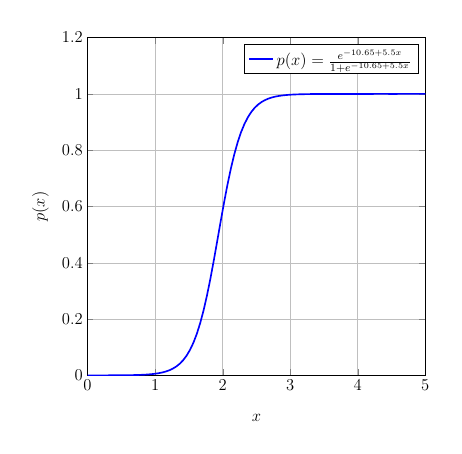
\begin{tikzpicture}[anchor = center, scale=.5]
    \begin{axis}[height=4in, width=4in,
      xmin=0,xmax=5,
      ymin=0,ymax=1.2,
      grid=major,samples=100,
      % grid style={line width=.5pt, draw=gray!50},
      % major grid style={line width=.8pt,draw=gray!90},
      % axis lines=middle,
      % minor tick num=5,
      % enlargelimits=true,%{abs=0.5},
      axis line style={-latex, thick},
      ticklabel style={font=\large},
      ylabel = {$p(x)$},
      xlabel = {$x$},
      % xlabel style={at={(ticklabel* cs:1)},anchor=north west},
      % ylabel style={at={(ticklabel* cs:1)},anchor=south west}
      x label style={at={(axis description cs:0.5,-0.1)},anchor=north,font=\large},
      y label style={at={(axis description cs:-0.1,.5)},rotate=0,anchor=south,font=\large},
      % legend pos= north east, clip = true
      ]
      \addplot+[no marks, very thick, blue,domain=0:5] { exp(-10.65 + 5.5*x)/(1 + exp(-10.65 + 5.5*x)};  \addlegendentry{\large $p(x) = \fr{e^{-10.65 + 5.5x}}{1 + e^{-10.65 + 5.5x}}$}
      % \only<4->{\addplot+[mark = +, thick,dashed, red] coordinates{ (10, 2.650) (30, 20.23) (70,53.55) (100,76.86) (130, 99.67)};  \addlegendentry{Lower 95\% confidence bound}}
    \end{axis}
  \end{tikzpicture}
  \pause \quad 
  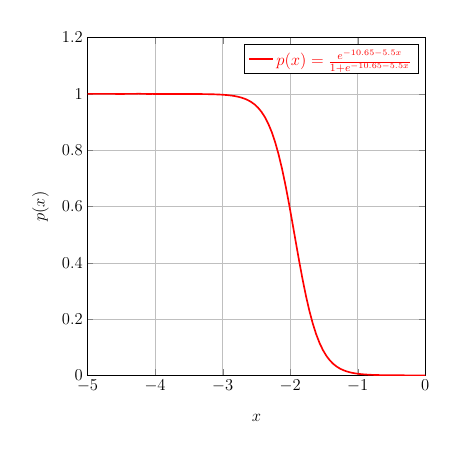
\begin{tikzpicture}[anchor= center,scale=.5]
    \begin{axis}[height=4in, width=4in,
      xmin=-5,xmax=0,
      ymin=0,ymax=1.2,
      grid=major,samples=100,
      % grid style={line width=.5pt, draw=gray!50},
      % major grid style={line width=.8pt,draw=gray!90},
      % axis lines=middle,
      % minor tick num=5,
      % enlargelimits=true,%{abs=0.5},
      axis line style={-latex, thick},
      ticklabel style={font=\large},
      ylabel = {$p(x)$},
      xlabel = {$x$},
      % xlabel style={at={(ticklabel* cs:1)},anchor=north west},
      % ylabel style={at={(ticklabel* cs:1)},anchor=south west}
      x label style={at={(axis description cs:0.5,-0.1)},anchor=north,font=\large},
      y label style={at={(axis description cs:-0.1,.5)},rotate=0,anchor=south,font=\large},
      % legend pos= north east, clip = true
      ]
      % \coordinate (O) at (0,0);
      % \node[fill=white,circle,inner sep=0pt] (O-label) at ($(O)+(-135:10pt)$) {$O$};
      \addplot+[no marks, very thick,red,domain=-5:0] { exp(-10.65 - 5.5*x)/(1 + exp(-10.65 - 5.5*x)};
      \addlegendentry{\rd \large $p(x) =  \fr{e^{-10.65 - 5.5x}}{1 + e^{-10.65 - 5.5x}}$}
    \end{axis}
  \end{tikzpicture}
  \pause
  
  What happens when $b$ is increased or decreased?
\end{frame}


\begin{frame}
  \frametitle{Logistic function (cont.)}
  \pause

  $b$ shifts the curve left or right (adjusts average fitted probabilities).\pause

  \bigskip
  
  \begin{tikzpicture}[anchor = center, scale=.5]
    \begin{axis}[height=4in, width=8in,
      xmin=-2,xmax=5,
      ymin=0,ymax=1,
      grid=major,samples=100,
      % grid style={line width=.5pt, draw=gray!50},
      % major grid style={line width=.8pt,draw=gray!90},
      % axis lines=middle,
      % minor tick num=5,
      % enlargelimits=true,%{abs=0.5},
      axis line style={-latex, thick},
      ticklabel style={font=\large},
      ylabel = {$p(x)$},
      xlabel = {$x$},
      % xlabel style={at={(ticklabel* cs:1)},anchor=north west},
      % ylabel style={at={(ticklabel* cs:1)},anchor=south west}
      x label style={at={(axis description cs:0.5,-0.1)},anchor=north,font=\large},
      y label style={at={(axis description cs:-0.1,.5)},rotate=0,anchor=south,font=\large},
      legend pos= north east, clip = true,
      legend style={row sep=5pt}
      ]
      \only<3->{\addplot+[no marks, very thick, blue,domain=-2:5] { exp(-10.65 + 5.5*x)/(1 + exp(-10.65 + 5.5*x)};  \addlegendentry{\bl \large $p(x) = \fr{e^{-10.65 + 5.5x}}{1 + e^{-10.65 + 5.5x}}$}}

      \only<4->{      \addplot+[no marks, very thick,red,domain=-2:5] { exp(0 + 5.5*x)/(1 + exp(0 + 5.5*x)};
      \addlegendentry{\rd \large $p(x) =  \fr{e^{0 + 5.5x}}{1 + e^{0 + 5.5x}}$}}
      % \only<4->{\addplot+[mark = +, thick,dashed, red] coordinates{ (10, 2.650) (30, 20.23) (70,53.55) (100,76.86) (130, 99.67)};  \addlegendentry{Lower 95\% confidence bound}}
    \end{axis}
  \end{tikzpicture}
  % \pause \quad 
  % \begin{tikzpicture}[anchor= center,scale=.5]
  %   \begin{axis}[height=4in, width=4in,
  %     xmin=-2,xmax=3,
  %     ymin=0,ymax=1.2,
  %     grid=major,samples=100,
  %     % grid style={line width=.5pt, draw=gray!50},
  %     % major grid style={line width=.8pt,draw=gray!90},
  %     % axis lines=middle,
  %     % minor tick num=5,
  %     % enlargelimits=true,%{abs=0.5},
  %     axis line style={-latex, thick},
  %     ticklabel style={font=\large},
  %     ylabel = {$p(x)$},
  %     xlabel = {$x$},
  %     % xlabel style={at={(ticklabel* cs:1)},anchor=north west},
  %     % ylabel style={at={(ticklabel* cs:1)},anchor=south west}
  %     x label style={at={(axis description cs:0.5,-0.1)},anchor=north,font=\large},
  %     y label style={at={(axis description cs:-0.1,.5)},rotate=0,anchor=south,font=\large},
  %     % legend pos= north east, clip = true
  %     ]
  %     % \coordinate (O) at (0,0);
  %     % \node[fill=white,circle,inner sep=0pt] (O-label) at ($(O)+(-135:10pt)$) {$O$};

  %   \end{axis}
  % \end{tikzpicture}
%  \pause
%  What happens when $\beta_0$ is increased or decreased?
\end{frame}


\begin{frame}
  \frametitle{Logistic function (cont.)}
  \pause

  $w_1$ adjusts the steepness of the curve: as $\beta_1$ increases, the curve becomes steeper
  \pause

  \medskip
  
  \begin{tikzpicture}[anchor = center, scale=.6]
    \begin{axis}[height=4in, width=7in,
      xmin=0,xmax=4,
      ymin=0,ymax=1,
      grid=major,samples=100,
      ytick={0,0.1,...,1},
      xtick={0,0.4,...,5.0},
      % grid style={line width=.5pt, draw=gray!50},
      % major grid style={line width=.8pt,draw=gray!90},
      % axis lines=middle,
      minor x tick num=25,
      % enlargelimits=true,%{abs=0.5},
      axis line style={-latex, thick},
      ticklabel style={font=\large},
      ylabel = {$p(x)$},
      xlabel = {$x$},
      % xlabel style={at={(ticklabel* cs:1)},anchor=north west},
      % ylabel style={at={(ticklabel* cs:1)},anchor=south west}
      x label style={at={(axis description cs:0.5,-0.1)},anchor=north,font=\large},
      y label style={at={(axis description cs:-0.1,.5)},rotate=0,anchor=south,font=\large},
      legend pos= north west, clip = true,
      legend style={row sep=5pt}
      ]
    \only<3->{ \addplot+[no marks, very thick, purple,domain=0:5] { exp(-10.65 + 3.5*x)/(1 + exp(-10.65 + 3.5*x)};  \addlegendentry{\Large $p(x) = \fr{e^{-10.65 + 3.5x}}{1 + e^{-10.65 + 3.5x}}$}}      
     \only<4->{\addplot+[no marks, very thick, orange,domain=0:5] { exp(-10.65 + 4.5*x)/(1 + exp(-10.65 + 4.5*x)};  \addlegendentry{\Large $p(x) = \fr{e^{-10.65 + 4.5x}}{1 + e^{-10.65 + 4.5x}}$}}
     \only<5->{ \addplot+[no marks, very thick, blue,domain=0:5] { exp(-10.65 + 5.5*x)/(1 + exp(-10.65 + 5.5*x)};  \addlegendentry{\Large $p(x) = \fr{e^{-10.65 + 5.5x}}{1 + e^{-10.65 + 5.5x}}$}}
     \only<6->{ \addplot+[no marks, very thick, red,domain=0:5] { exp(-10.65 + 6.5*x)/(1 + exp(-10.65 + 6.5*x)};  \addlegendentry{\Large $p(x) = \fr{e^{-10.65 + 6.5x}}{1 + e^{-10.65 + 6.5x}}$}}
     \only<7->{  \addplot+[no marks, very thick, green,domain=0:5] { exp(-10.65 + 7.5*x)/(1 + exp(-10.65 + 7.5*x)};  \addlegendentry{\Large $p(x) = \fr{e^{-10.65 + 7.5x}}{1 + e^{-10.65 + 7.5x}}$}}
      % \only<4->{\addplot+[mark = +, thick,dashed, red] coordinates{ (10, 2.650) (30, 20.23) (70,53.55) (100,76.86) (130, 99.67)};  \addlegendentry{Lower 95\% confidence bound}}
    \end{axis}
  \end{tikzpicture}
 
\end{frame}


\begin{frame}
  \frametitle{Odds ratio and the logit function}\pause
  From the logistic function, we can obtain the \textbf{\bl odds ratio} ($OR$) as:
  \pause
  \begin{equation}
    \label{eq:2}\bl
    OR = \fr{p( x)}{1 - p(\bm x)} = e^{b + w_1x}
  \end{equation}
  which is considered as the relative likelihood of success ($p(x)$).\pause

  \bigskip

  Taking the log of the odds ratio yields the log-odds or \textbf{\dca logit} function:
  \pause
  \begin{equation}
    \label{eq:3}
    \dca logit(p(x)) = \pause \log\lt(\fr{p(\bm x)}{1 - p( x)}\rt) =
    b + w_1  x
  \end{equation}
  \pause
  \begin{alertblock}{Notes}\pause
    \begin{itemize}[<+->]
    \item The logit function is linear in $x$
    \item The inverse of the logit function yields the logistic function
    \item In the generalized linear framework, logit is the \textit{link function} between the predictors and the mean response
    \end{itemize}
  \end{alertblock}
\end{frame}

\section{Logistic regression model}

\begin{frame}
  \frametitle{Logistic regression}
  Logistic regression is an approach for modeling the \textit{probability} of a \textit{multinomial} response.\pause

  \bigskip
  
  In the simple case, we consider a binomial (or binary) response.\pause

  \begin{block}{Logistic function}
    This is the model equation for simple logistic regression:\pause
    \begin{equation}
      \label{eq:1}
      p(y=1|\bm x;\bm\th) = \fr{e^{b + w_1 x}}{1 + e^{b + w_1X}}
    \end{equation}
    \pause where $p(y=1|\bm x,\bm\th) \in [0,1]$
  \end{block}

  \pause
  {\rd The logistic function is a member of the class of \textbf{sigmoid} functions (S-shaped curves) and can also be written:\pause
    \begin{equation}
      p(y=1|x,\bm\th) = \fr{1}{1 + e^{-\bm w\tr\bm x}} \pause = 
      (1 + e^{-\bm w\tr\bm x})^{-1} \pause = \sigma(\bm w\tr\bm x)
    \end{equation}
    \pause
    where $\bm w\tr = (b,w_1)$
  }
\end{frame}


\begin{frame}
    \frametitle{Example 1: Binomial logistic regression with single predictor}
\pause
    \begin{exampleblock}{Credit card defaults}\pause
      \begin{itemize}
      \item Data:  A simulated data set containing information on ten thousand customers.\pause
      \item Question: Can we predict which customers will default on their credit card debt (based on income, etc)?
  \end{itemize}

  \end{exampleblock}
  
  \bigskip
  Four variables: \pause
  \begin{itemize}[<+->]
  \item \texttt{\bl default}:
    A factor with levels \textit{No} and \textit{Yes} indicating whether the customer defaulted on their debt
  \item \texttt{\bl student}: A factor with levels \textit{No} and \textit{Yes} indicating whether the customer is a student 
  \item \texttt{\bl balance}: The average balance that the customer has remaining on their credit card after making their monthly payment
  \item \texttt{\bl income}:  Income of customer
  \end{itemize}
\end{frame}

\begin{frame}[fragile,fragile]
  \frametitle{Example 1: Binomial logistic regression (cont.)}\pause
  We want to model the probability of \texttt{\bl default} based on the \texttt{\bl balance} predictor. \pause

 
  The estimated coefficients from a computer program are: \pause
  
  {\bl
\begin{verbatim}
              Estimate Std. Error z value Pr(>|z|)    
(Intercept) -1.065e+01  3.612e-01  -29.49   <2e-16 ***
balance      5.499e-03  2.204e-04   24.95   <2e-16 *** 
\end{verbatim}
}
\pause
Note that the null hypothesis for the tests is: $H_0 : \bm w_i = 0$ (i.e.\ no dependence on the corresponding predictor)
\end{frame}

\begin{frame}
  \frametitle{Example 1: Binomial logistic regression (cont.)}\pause
  The estimated model is: \pause

  \begin{equation}
    \bl  \hat p(y=1|\bm x;\bm \th) = \fr{e^{(-10.65 + 0.0055x)}}{1 + e^{(-10.65 + 0.0055x)}} = \pause
    \fr{1}{1 + e^{(10.65 - 0.0055x)}} = \pause \sigma(1 + e^{(10.65 - 0.0055x)})
  \end{equation}
  \pause
  % \vspace{-2ex}
  
  \begin{figure}[h!]
    \centering
    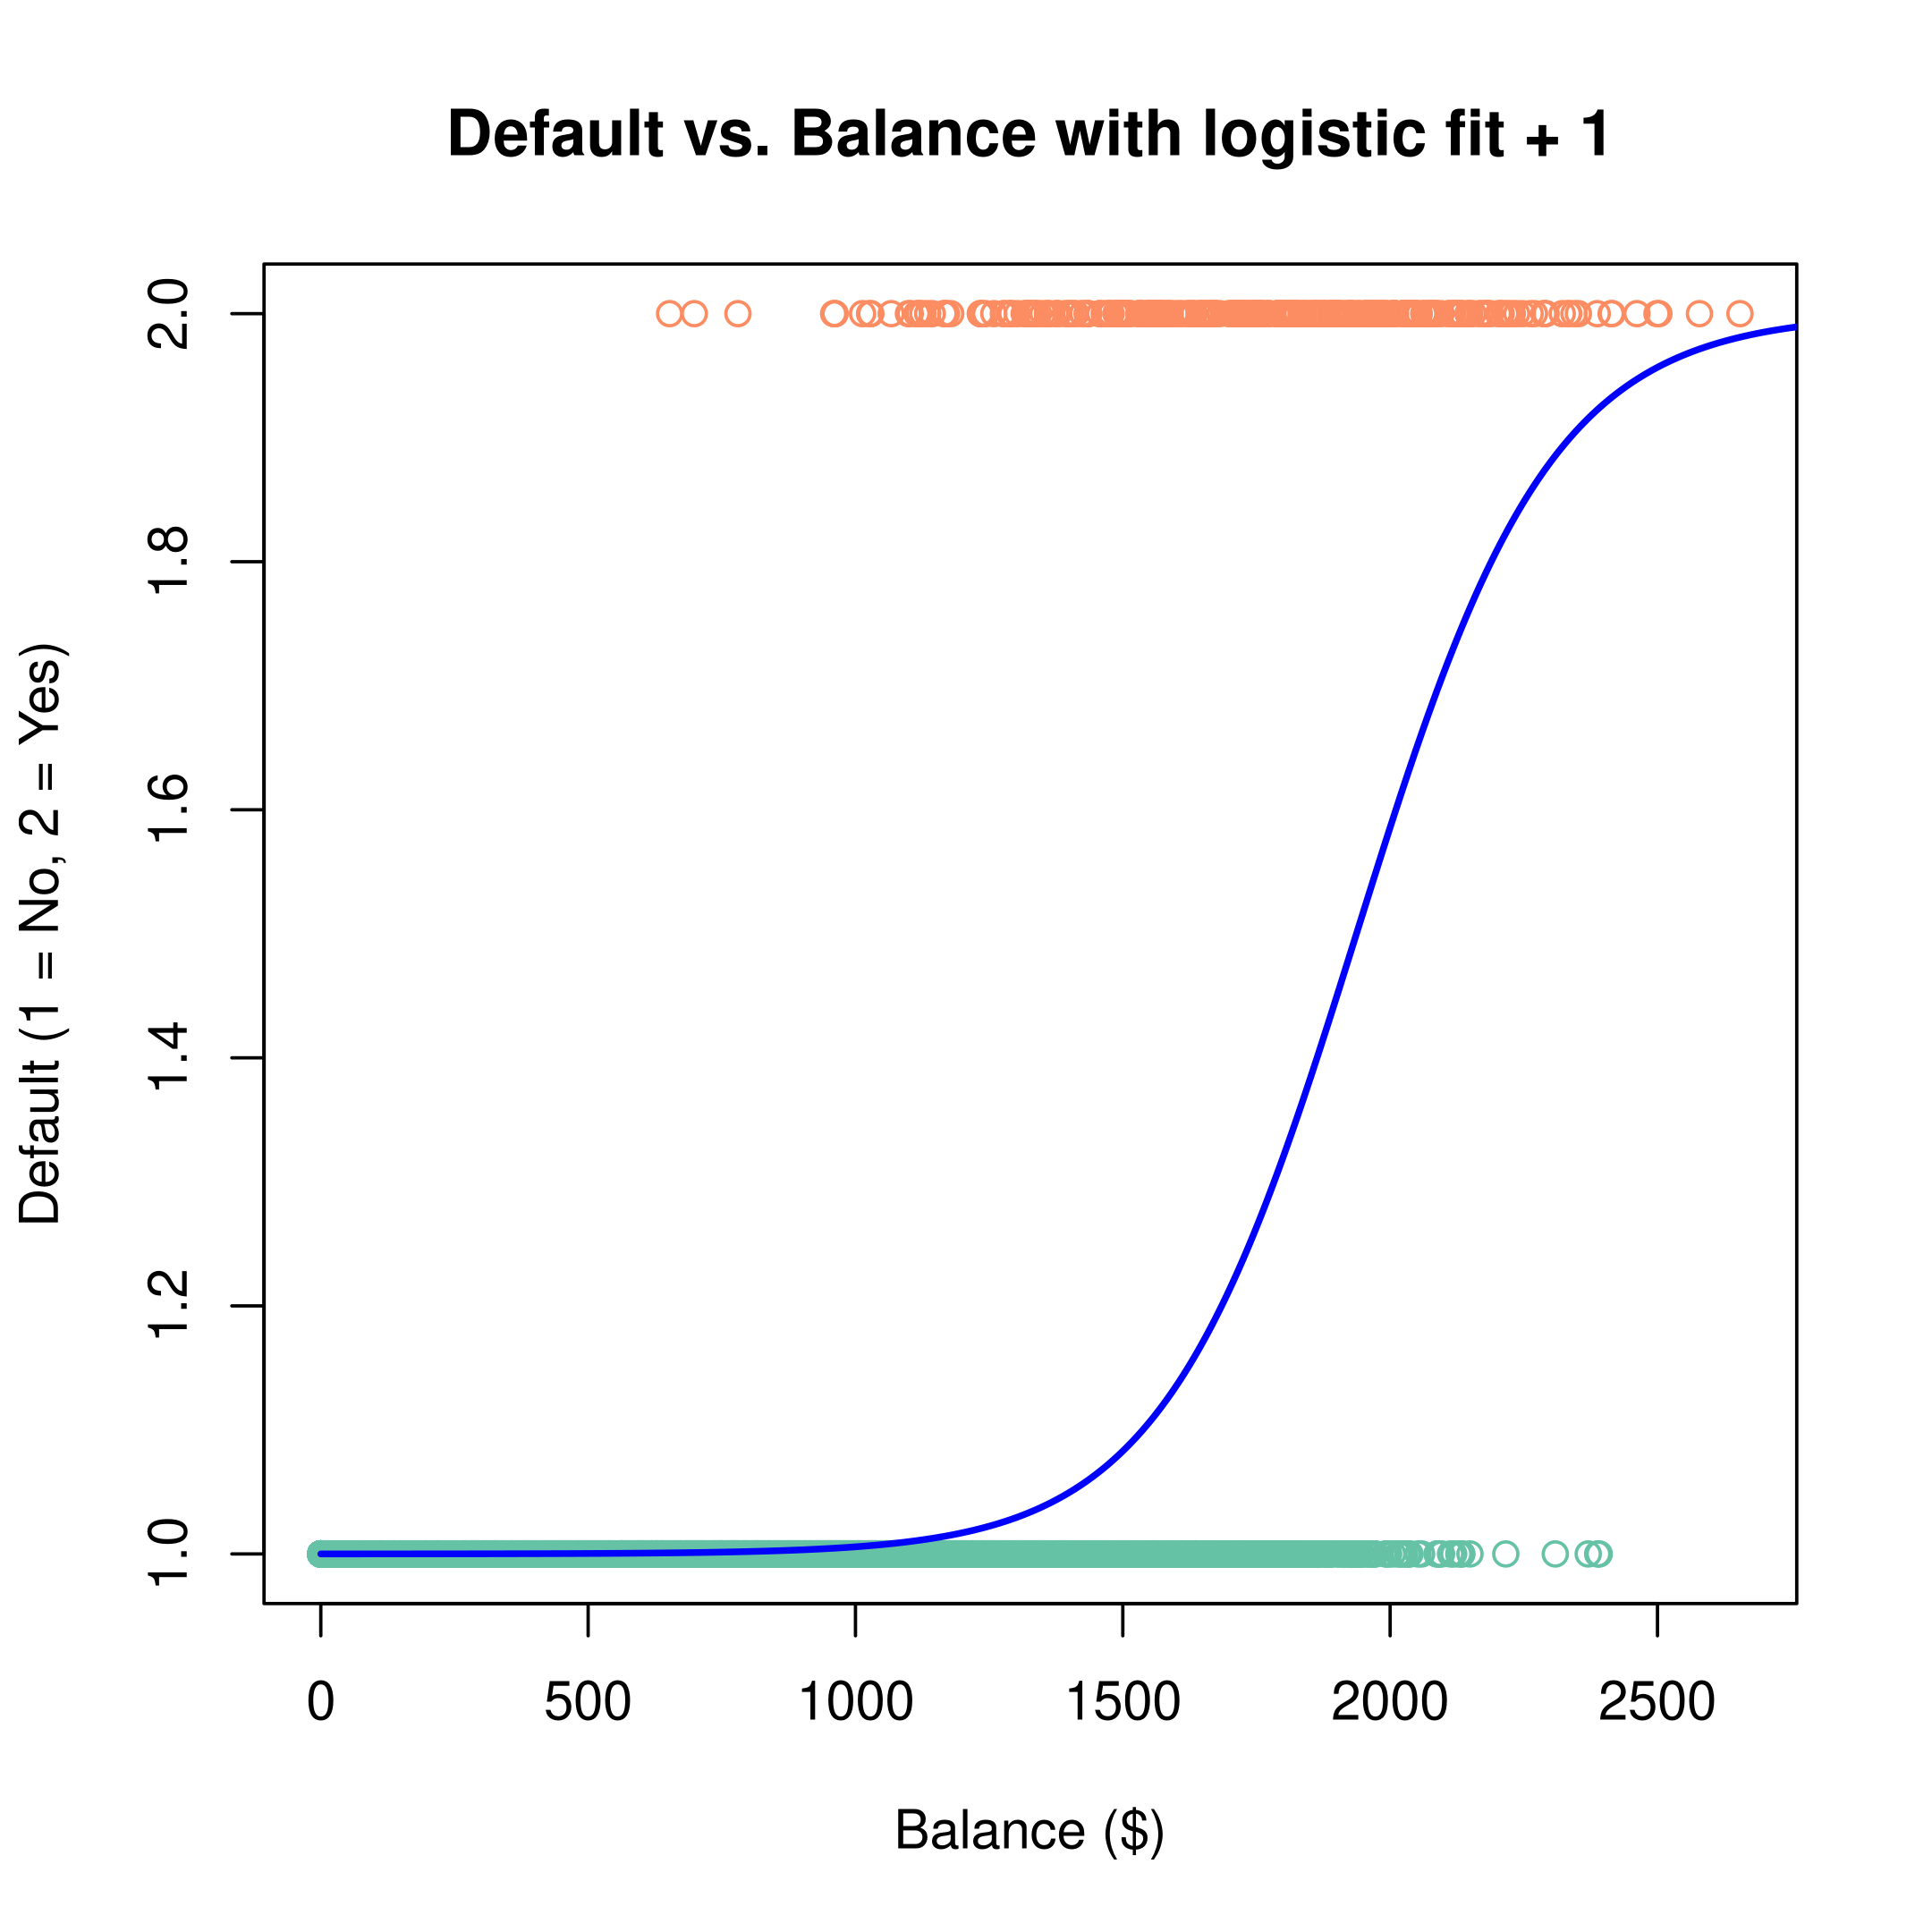
\includegraphics[width=.4\textwidth]{income-balance-model}
    \caption{Logistic regression model predicting the probability of \texttt{\bl default} based on \texttt{\bl balance}.
    The blue line is the estimated function $\hat p(\bm x)$. The scatterplot uses a 1/2 encoding.}
  \end{figure}
\end{frame}


\begin{frame}
  \frametitle{Example 1: Binomial logistic regression (cont.)}
  \pause
  Recall the model:\pause
  \begin{equation*}
    \hat p(y=1|x) = \fr{e^{-10.65 + 0.0055x}}{1 + e^{-10.65 + 0.0055x}}
  \end{equation*}
  \pause
  \begin{enumerate}[<+->]
  \item How would $\hat p$ (the predicted probability) change if $x$ were to increase by \$100?
  \item What about if $x$ were to decrease by \$100
  \item There are 333 defaults out of 10000 observations. What is the impact of $b$?
  \end{enumerate}
\end{frame}

\begin{frame}
  \frametitle{Multiple logistic regression}\pause
  In multiple logistic regression, we predict a binary response using \textit{multiple predictors}:\pause
  \begin{equation}
    \label{eq:37}
    \log\lt( \fr{p(x)}{1 - p(x)} \rt) = \pause b + w_1 x_1 + \cdots + \bm w_Dx_D = \pause \bm w\tr X
  \end{equation}
  \pause
  where $\bm x = (x_1, \ldots, x_D)$.

  \pause

  \begin{exampleblock}{Activity: Binomial logistic regression with multiple predictors}
  Using the \texttt{Default} dataset, predict the probability of \texttt{\bl default} based on \texttt{\bl balance}
  and \texttt{\bl student}. Comment on your results and interpret the coefficient estimates.

    \begin{center}
    \includegraphics<3->[width=.3\textwidth]{income-balance}
  \end{center}
\end{exampleblock}
\end{frame}


\begin{frame}
  \frametitle{Decision boundary}
  \pe
  This is the line that defines the probability threshold $\tau$ for class assignment:\pe

  In 1-D: \pe
  \begin{equation}
   x^{*}: p(y=1|x = x^{*},\bm \th) = \tau
 \end{equation}
 \pe
 Typically, $\tau = 0.5$
 
\end{frame}

\section{MLE}
\begin{frame}
  \frametitle{Estimation of logistic regression coefficients}
  \pause

  The method of \textbf{\bl maximum likelihood} is used to estimate logistic regression coefficients $\bm w$ \pause
  \begin{itemize}[<+->]
  \item The likelihood function $\bl \mathcal{L}(\theta)$ represents the support provided by a sample for a given parameter $\theta$:\pause
    \begin{equation}
      \label{eq:4}
      \bl \mathcal{L}(\bm\theta) = \prod_{i=1}^N p_{c_i}(x_i;\bm\theta)
    \end{equation}
    \pause
    
    \begin{itemize}
    \item where   $p_{c_i}(x_i;\bm\theta) = \Pr(G = c_i|X = x_i;\bm\theta)$
    \item In the two-class case: $\bm\theta = \bm w = \{b,w_1\}$
    \end{itemize}

 
  \item Thus, we can write the conditional probabilities as:\pause
    \begin{align}
      \label{eq:6}
      p_1(x;\bm\theta) &= p(x;\bm\theta)\\
      p_2(x;\bm\theta) &= 1 - p(x;\bm\theta)
    \end{align}

  \item It is also convenient to encode $c_i$ using a 0/1 response $y_i$:\pause
    \begin{equation}
      \label{eq:5}
      y_i =
      \begin{cases}
        1, & \text{when } c_i = \text{Class } 1\\
        0, & \text{when } c_i = \text{Class } 2
      \end{cases}
    \end{equation}
  \end{itemize}
\end{frame}


\begin{frame}
  \frametitle{Log-likelihood function for logistic regression}\pause

  The principle of maximum likelihood dictates that the best parameter estimates are those that maximize the likelihood function. \pause

  
  \begin{itemize}
  \item Equivalently, we \textit{minimize} the \textbf{\rd negative log-likelihood} function $\text{NLL}(\bm\theta)$:
    \pause
  \begin{equation}
    \rd \text{NLL}(\bm\theta) =- \sum_i \log p_{c_i}(x_i;\bm\theta)
  \end{equation}\pause

\item In the binomial case, this simplifies to:\pause
  \begin{equation}
    \label{eq:7}
    \text{NLL}(\bm w)= -\sum_i \lt[ y_i \log p(x_i;\bm w) + (1-y_i)\log(1-p(x_i;\bm w))\rt]               
  \end{equation}
  \pause

  \item Recall that we model $p(x_i;\bm w)$ as:\pause
  \begin{equation}
    \label{eq:8}
    p(x_i) = \fr{e^{b + w_1x_i}}{1 + e^{b + w_1x_i}}          
  \end{equation}
\end{itemize}

\end{frame}



\begin{frame}
  \frametitle{Log-likelihood function for logistic regression}\pause
  Substituting \eqref{eq:8} into \eqref{eq:7}, we obtain:\pause
  \begin{eqnarray}
    \label{eq:9}
    \begin{split}
      \text{NLL}(\bm w) &= -\sum_i\lt[ {\pl y_i\log\lt( \fr{e^{b + w_1x_i}}{1 + e^{b + w_1x_i}} \rt)} +
        {\gr(1-y_i)\log\lt( 1- \fr{e^{b + w_1x_i}}{1 + e^{b + w_1x_i}} \rt)}\rt]\\ \pause
        &= -\sum_i\lt[{\pl y_i\log\lt( \fr{e^{b + w_1x_i}}{1 + e^{b + w_1x_i}} \rt) }+
        {\gr (1-y_i)\log\lt( \fr{1}{1 + e^{b + w_1x_i}} \rt)}        \rt]\\ \pause
        &=- \sum_i\Big[
        {\pl y_i \log \lt( e^{b + w_1x_i}\rt) - y_i\log\lt(1 + e^{b + w_1x_i}\rt)}\\ \pause
        & \qquad \qquad + {\gr \cancelto<6->{0}{(1-y_i)\log(1)}  -(1-y_i)\log\lt(1 + e^{b + w_1x_i}\rt)} \Big]\\ \pause
        &= -\sum_i\Big[
        y_i\lt(b + w_1x_i \rt) \cancelto<9->{}{ -y_i\log\lt(1 + e^{b + w_1x_i}\rt)}
        -\log\lt(1 + e^{b + w_1x_i}\rt) \\ \pause
        &\qquad \qquad \cancelto<10->{}{+ y_i\lt(1 + e^{b + w_1x_i}\rt)}
        \Big]\\\pause
        \bl \text{NLL}(\bm w)    &= -\sum_i \lt[ y_i\lt(b + w_1x_i \rt) - \log\lt(1 + e^{b + w_1x_i}\rt) \rt]
    \end{split}
  \end{eqnarray}
\end{frame}

\begin{frame}
  \frametitle{Maximizing the log-likelihood}\pause
  To find $\hat{\bm w}$, we find the derivative of $\text{NLL}(\bm w)$, set it to zero and solve the resulting \textbf{\dca score equations}:\pause
  \begin{eqnarray}
    \label{eq:10}
    \begin{split}
      \pd{\text{NLL}}{\bm w}
      &=- \pd{}{\bm w}\sum_i \lt[ y_i\lt(b + w_1x_i \rt) - \log\lt(1 + e^{b + w_1x_i}\rt) \rt]\\ \pause
      \begin{pmatrix}
        {\pl \pd{\text{NLL}}{b}}\\[3mm]
        {\gr \pd{\text{NLL}}{w_1}}
      \end{pmatrix}
      &=-
      \begin{pmatrix}
        {\pl \sum_i \lt[ y_i    - \fr{e^{b + w_1x_i}}{1 + e^{b + w_1x_i}}\rt]} \\[3mm]
        {\gr \sum_i \lt[ x_iy_i - \fr{x_i\lt(e^{b + w_1x_i}\rt)}{1 + e^{b + w_1x_i}}\rt] }
      \end{pmatrix} \\[2mm]\pause
      \begin{pmatrix}
        {\pl \pd{\text{NLL}}{b}}\\[3mm]
        {\gr \pd{\text{NLL}}{w_1}}
      \end{pmatrix}
      &= -
      \begin{pmatrix}
        {\pl \sum_i \lt[y_i - p(x_i) \rt]}\\[3mm]
        {\gr \sum_i \lt[ x_i\lt(y_i - p(x_i)\rt)\rt] }
      \end{pmatrix}\pause
      =
      \begin{pmatrix}
        0 \\[3mm] 0
      \end{pmatrix}
    \end{split}    
  \end{eqnarray}
  \pause
  This is a system of two \textit{\rd nonlinear} equations in $\bm w$ \pause which can be solved via the
  \textbf{Newton-Raphson} method. \pause

  \bigskip
  
  Alternatively, we can use the \textbf{gradient descent} approach to directly minimize $\text{NLL}$.
\end{frame}

\begin{frame}
  \frametitle{Maximum likelihood estimation (MLE) in logistic
    regression}\pause

  Recall the negative log-likelihood function for the binomial logistic regression case: \pause
  \begin{equation}
    \label{eq:16}
    \bl \text{NLL}(\bm w) = -\sum_i \lt[ y_i\lt(b + w_1x_i \rt) - \log\lt(1 + e^{b + w_1x_i}\rt) \rt]
  \end{equation}
  \pause
  The optimal $\hat{\bm w}$ which minimizes $\text{NLL}(\bm w)$ is the \textbf{\dca maximum likelihood estimate}.

  \pause

  \bigskip

  Also recall the derivative of $ \text{NLL}$: \pause
  \begin{equation}
    \label{eq:17}
    \nabla_{\bm w}\text{NLL} = \pause
    \begin{pmatrix}
      {\pl \pd{ \text{NLL}}{b}}\\[3mm]
      {\gr \pd{ \text{NLL}}{w_1}}
    \end{pmatrix} = \pause
    \begin{pmatrix}
    -  \pl \sum_i \lt[y_i - p(x_i) \rt]\\[3mm]
     - \gr \sum_i \lt[ x_i\lt(y_i - p(x_i)\rt)\rt] 
    \end{pmatrix}
  \end{equation}
  \pause
  We can use either Newton-Raphson or gradient \textit{\rd descent} to \textit{\rd minimize} $ \text{NLL}$.
\end{frame}


\begin{frame}
  \frametitle{NLL and entropy}
  \pe
  We can show that the NLL is equal to the sum of the \textbf{binary cross entropy} of $y_i$ and $p(y=1|\bm x_i)$ over $N$:\pe
  \begin{equation}
    \mb{H}_i(y_i,p_i) = - [y_i\log p_i + (1-y_i)\log(1-p_i)]
  \end{equation}
  \pe
  Note that $p_i = \bm\si(\bm w\tr \bm x_i)$.
  \begin{itemize}
    \item Binary cross-entropy quantifies how far your predicted probabilities are from the actual binary labels.
  \end{itemize}
\end{frame}

\begin{frame}
  \frametitle{Binary Cross Entropy vs. p (when y=1)}
  \pe
  For a true label $y=1$, the binary cross entropy is $\mb{H}(1,p) = -\log(p)$. \pe
  This function penalizes predictions that are far from the true label:
  
  \begin{center}
  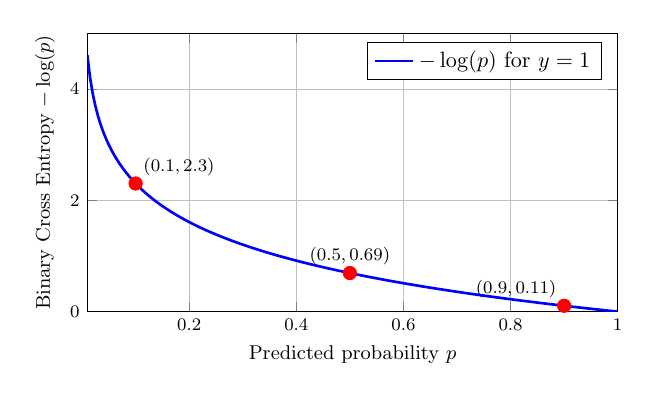
\begin{tikzpicture}[scale=0.8]
    \begin{axis}[
      width=10cm,
      height=6cm,
      xlabel={Predicted probability $p$},
      ylabel={Binary Cross Entropy $-\log(p)$},
      xmin=0.01, xmax=1,
      ymin=0, ymax=5,
      grid=major,
      samples=200,
      axis line style={-latex},
      ticklabel style={font=\footnotesize},
      xlabel style={font=\small},
      ylabel style={font=\small},
      legend pos=north east
    ]
    \addplot[blue, very thick, domain=0.01:1] {-ln(x)};
    \addlegendentry{$-\log(p)$ for $y=1$}
    
    % Add some key points
    \addplot[red, only marks, mark=*, mark size=3pt] coordinates {
      (0.1, {-ln(0.1)})
      (0.5, {-ln(0.5)})
      (0.9, {-ln(0.9)})
    };
    
    % Add annotations
    \node[anchor=south west] at (axis cs:0.1, {-ln(0.1)}) {\footnotesize $(0.1, 2.3)$};
    \node[anchor=south] at (axis cs:0.5, {-ln(0.5)}) {\footnotesize $(0.5, 0.69)$};
    \node[anchor=south east] at (axis cs:0.9, {-ln(0.9)}) {\footnotesize $(0.9, 0.11)$};
    \end{axis}
  \end{tikzpicture}
  \end{center}
  
  \pe
  \textbf{Key observations:}
  \begin{itemize}[<+->]
    \item As $p \to 1$: cross entropy $\to 0$ (low penalty for correct prediction)
    \item As $p \to 0$: cross entropy $\to \infty$ (high penalty for incorrect prediction)
    \item The function is convex, ensuring unique minimum in optimization
  \end{itemize}
\end{frame}

\begin{frame}
  \frametitle{Example: predicting spam}

  \pause
  \begin{enumerate}[\bf (a)]
    \item If the email is spam (y=1) and you predict 90\% probability of spam (p=0.9), find the binary cross entropy (BCE):\pause
    \[
    \text{BCE} = -[1 \times \log(0.9) + 0 \times \log(0.1)] = -\log(0.9) \approx 0.105 \quad (\text{low loss - good!})
    \] \pause
    \item If the email is spam (y=1) but you predict only 10\% probability of spam (p=0.1), find the BCE. \pause
    \[
    \text{BCE} = -[1 \times \log(0.1) + 0 \times \log(0.9)] = -\log(0.1) \approx 2.303 \quad (\text{high loss - bad!})
    \]
  \end{enumerate}

\end{frame}

\section{Optimization}
\begin{frame}
  \frametitle{Gradient descent for MLE in logistic regression}
  \pause

  This approach only requires the first derivative:\pause
  \begin{equation}
    \label{eq:24}
    \bm w_{k+1} = \bm w_k - \rho\nabla\text{NLL}(\bm w_k)
  \end{equation}\pause
  Thus, to find $\hat{\bm w}$ we iterate using:
  \pause
  \begin{equation}
    \label{eq:25}
    \begin{pmatrix}
      \bm w_{0,k} \\ \bm w_{1,k}
    \end{pmatrix}
    = \pause
    \begin{pmatrix}
      \bm w_{0,k} \\ \bm w_{1,k}
    \end{pmatrix}
    {\bl +} ~ \rho
    \begin{pmatrix}
      \pl \sum_i \lt[y_i - p(x_i) \rt]\\[3mm]
      \gr \sum_i \lt[ x_i\lt(y_i - p(x_i)\rt)\rt] 
    \end{pmatrix}
  \end{equation}\pause
  
  Because the negative log-likelihood is \textit{\bl convex}, and thus a \textit{\bl minimization} problem,
  we \textit{\bl descend} the function and thus
  \textit{\bl subtract} the scaled derivative.\pause

  
  \begin{alertblock}{Note}
  \begin{itemize}[<+->]
  \item The gradient descent method does not require a second derivative
  \item However, it may require more iterations to converge than Newton-Raphson
  \end{itemize}
\end{alertblock}

  
\end{frame}

\begin{frame}
  \frametitle{Newton-Raphson approach for MLE in logistic regression}\pause
    The optimal point $\hat{\bm w}$ is given by the root of the equation $\nabla_{\bm w}\text{NLL} = 0$.\pause

    \bigskip
    
    Applying Newton-Raphson, the update step is:\pause
    \begin{equation}
      \label{eq:nr}
      \bm w_{k+1} = \bm w_k - {\bm H}^{-1}_{\bm w_k}(\text{NLL})\nabla_{\bm w_k}\text{NLL}(\bm w_k)
    \end{equation}
    \pause
    The operator $\bm H^{-1}$ represents the inverse \textbf{Hessian} (second derivative) matrix of $\text{NLL}$ with respect to
    $\bm w$: \pause
    \begin{equation}
      \label{eq:19}
      {\bm H}_{\bm w_k}(\text{NLL}) =\nabla_{\bm w_k}^2\text{NLL}=
      \begin{pmatrix}
        \rd \pdd{\text{NLL}(\bm w)}{b} & \pl \pd{^2\text{NLL}(\bm w)}{bw_1} \\[2mm]
        \pl \pd{^2\text{NLL}(\bm w)}{w_1b} &  \bl \pdd{\text{NLL}(\bm w)}{w_1}\\
      \end{pmatrix}
    \end{equation}\pause
    Note that  \eqref{eq:nr} is just the matrix representation of the 1-D case: \pause
    \begin{equation}
    \bm w_{k+1} =\bm w_k - \fr{\text{NLL}'(\bm w_k)}{\text{NLL}''(\bm w_k)}\label{eq:21}
  \end{equation}

\end{frame}

\begin{frame}
  \frametitle{Newton-Raphson approach for MLE (cont.)}\pause
  We can work out each component of the second derivative: \pause
  \begin{eqnarray}
    \label{eq:20}
    \rd \pdd{\text{NLL}(\bm w)}{b} & \rd =& \rd  \sum_i p(x_i)(1 - p(x_i)) \\\pause
    \pl \pd{^2\text{NLL}(\bm w)}{bw_1} & \pl =& \pl  \sum_i x_i p(x_i)(1 - p(x_i)) \\\pause
    \bl \pdd{\text{NLL}(\bm w)}{w_1} & \bl =& \bl  \sum_ix_i^2 p(x_i)(1 - p(x_i)) 
  \end{eqnarray}
  \pause
  The complete update can then be shown as:\pause
  \begin{equation}
    \label{eq:22}
    \begin{pmatrix}
      \bm w_{0,k+1}\\[3mm]
      \bm w_{1,k+1}    
    \end{pmatrix}
     = \pause
    \begin{pmatrix}
      \bm w_{0,k}\\[3mm]
      \bm w_{1,k}
    \end{pmatrix}  - \pause
    \lt[
    \begin{pmatrix}
      \rd \pdd{\text{NLL}(\bm w)}{b} & \pl \pde{\text{NLL}(\bm w)}{b}{w_1} \\[2mm]
      \pl \pde{\text{NLL}(\bm w)}{w_1}{b} &  \bl \pdd{\text{NLL}(\bm w)}{w_1}
    \end{pmatrix}^{-1}
    \begin{pmatrix}
      \pl \pd{\text{NLL}}{b}\\[2mm]
      \gr \pd{\text{NLL}}{w_1}
    \end{pmatrix}\rt]_{\bm w_k}
  \end{equation}\pause
  Alternatively:\pause
  \begin{equation}
    \label{eq:28}
    \bm w_{k+1}  = \bm w_k - \lt[\lt(\pde{\text{NLL}(\bm w)}{\bm w}{\bm w\tr}\rt)^{-1} \pd{\text{NLL}(\bm w)}{\bm w}\rt]_{\bm w_k}
  \end{equation}
\end{frame}

\begin{frame}
  \frametitle{Compact matrix representation of derivatives}
  \pause
  Recall in 1D: \pause
  $ \bm w =
    \begin{pmatrix}
      b \\ w_1
    \end{pmatrix}$. \pause 
  If we denote:
$    \bm x_i =
    \begin{pmatrix}
      1 \\ x_i
    \end{pmatrix}
$
\pause
Then we can write:\pause
\begin{equation}
  \label{eq:31}
  \begin{split}
  \pd{\text{NLL}(\bm w)}{\bm w} &=
  \begin{pmatrix}
    -\sum_i \lt[y_i - p(x_i) \rt]\\[3mm]
    - \sum_i \lt[ x_i\lt(y_i - p(x_i)\rt)\rt] 
  \end{pmatrix} \pause =
 - \begin{pmatrix}
    1 & x_1 \\
    1 & x_2 \\
    \vdots & \vdots \\
    1 & x_n
  \end{pmatrix}^T\pause
  \begin{pmatrix}
    y_1 - p(x_1)\\
    y_2 - p(x_2)\\
    \vdots \\
    y_n - p(x_n)
  \end{pmatrix}\\
  \pause &= -\bm{X}^T(\bm y - \bm p)
\end{split}
\end{equation}
\end{frame}

\begin{frame}
  \frametitle{Compact matrix representation of derivatives (cont.)}
  \pause
  We can also decompose the Hessian as: \pause
  \begin{equation}
    \label{eq:32}
    \begin{split}
    \pde{\text{NLL}(\bm w)}{\bm w}{\bm w\tr} &=
    \begin{pmatrix}
       \sum_i p(x_i)(1 - p(x_i)) & \sum_i x_i p(x_i)(1 - p(x_i)) \\
     \sum_i x_i p(x_i)(1 - p(x_i)) &   \sum_ix_i^2 p(x_i)(1 - p(x_i)) 
   \end{pmatrix}\\[2mm]
   &= \bm X^T\bm S \bm X
 \end{split}
\end{equation}
\pause
where $\bm S$ is a diagonal $N\times N$ matrix:\pause
\begin{equation}
  \label{eq:33}
  \bm S =
  \begin{pmatrix}
    p(x_1)(1 - p(x_1)) & 0 & \ldots & 0 \\
    0 & p(x_2)(1 - p(x_2)) & \ldots & 0 \\
    \vdots & \vdots & \ddots & 0 \\
    0 & 0 & 0 & p(x_n)(1 - p(x_n))
  \end{pmatrix}
\end{equation}
\pause
and $\bm X$ is defined as before:\pause
\begin{equation}
  \bm X^T =
  \begin{pmatrix}
    1 & 1 & \cdots & 1 \\
    x_1 &x_2 & \cdots & x_n
  \end{pmatrix}
\end{equation}
\end{frame}

\begin{frame}
  \frametitle{Compact matrix representation (cont.)}
  \label{appendix-label}
  \pause
  Putting the previous results together, we can express the update step as:\pause
  \begin{align}
    \label{eq:34}
    \begin{split}
      \bm w_{k+1} &= \bm w_{k} - \bm H^{-1}\bm g_k\\\pause
       &= \bm w_{k} + (\bm X^T \bm W \bm X)^{-1}\bm X\tr (\bm y - \bm p) \\\pause
      &= {\og (\bm X^T \bm W \bm X)^{-1}} {\pl (\bm X^T \bm W \bm X)} \bm w_{k} + \pause
      {\og (\bm X^T \bm W \bm X)^{-1}} {\pl \bm X^T} (\bm y - \bm p) \\\pause
      &= {\og (\bm X^T \bm W \bm X)^{-1}}{\pl \bm X^T \bm W }\lt( {\pl \bm X} \bm w_k
      + {\pl \bm W^{-1} }(\bm y - \bm p)  \rt)\\\pause
      &= (\bm X^T \bm W \bm X)^{-1} \bm X^T \bm W {\gr \bm z}
    \end{split}
  \end{align}
  \pause
  where the adjusted response $\bm z$ is given as:
  \pause
  \begin{equation}
    \label{eq:35}
    \gr\bm z = \bm X\bm w_k + \bm W^{-1} (\bm y - \bm p)
  \end{equation}
  \pause
  In this form, the estimation is also called iteratively reweighted least squares
  (IRLS).  %\hyperlink{summary-cont}{\beamerbutton{Back}}
\end{frame}



 \begin{frame}
  \frametitle{OLS, WLS and IRLS}\pause

    \begin{itemize}
    \item  Recall the OLS estimate:
      \begin{equation}
        \hat{\bm w} = (\bm X^T\bm X)^{-1}\bm X^T\bm y
      \end{equation}
      \pause
      if $\bm y$ is the response.\pause

    \item Also recall that the weighted least squares (WLS) is given by:

      \begin{equation}
      \hat{\bm w} = (\bm X^T\bm W \bm  X)^{-1}\bm X^T \bm W y
    \end{equation}
    \pause
    

  \item In logistic regression, the coefficients can be found via the Newton-Raphson update, which can be specified as:
    \pause 
  \begin{equation}
       \bm w_{k+1} 
        = (\bm X^T \bm W \bm X)^{-1} \bm X^T \bm W {\gr \bm z}
  \end{equation}
  \pause
  where $\bm z$ is given as:
  \begin{equation}
    \label{eq:35}
    \gr\bm z = \bm X\bm w_k + \bm W^{-1} (\bm y - \bm p)
  \end{equation}
  \pause
  \begin{itemize}
  \item Note that the update step is identical in form to the WLS estimator
  \item  However, $\bm W$ and $\bm z$ change in each iteration, hence the name iteratively reweighted least squares (IRLS)

  \end{itemize}
   \end{itemize}
 
\end{frame}




\section{Outlook}

\begin{frame}
  \frametitle{Summary}
  \begin{itemize}
  \item The binary logistic regression model is given by:
      \begin{equation}
      \label{eq:1}
      p(y=1|\bm x;\bm \th) = \fr{1}{1 + e^{-\bm w\tr \bm x}}
    \end{equation}
  \item   The negative log-likelihood of a sample of $N$ observations in the binomial response case is:
    \begin{equation}
     \text{NLL}(\bm w) = \sum_i \lt[ y_i\lt(b + w_1x_i \rt) - \log\lt(1 + e^{b + w_1x_i}\rt) \rt]
   \end{equation}
   \item Based on the principle of maximum likelihood, the estimate $\hat{\bm w}$ is given by the minimizing $\text{NLL}$.

\item    This can be solved via gradient descent or Newton-Raphson.
 \end{itemize}

 \end{frame}

 \begin{frame}
   \frametitle{Summary (cont.)}
   \label{summary-cont}
   \textbf{Gradient descent update for logistic regression}
   \begin{equation}
     \bm w_{k+1} = \bm w_k - \lambda\nabla\text{NLL}(\bm w_k)
   \end{equation}

   \textbf{Newton-Raphson update for logistic regression}
   \begin{equation}
      \bm w_{k+1} = \bm w_k - {\bm H}^{-1}_{\bm w_k}(\text{NLL})\nabla_{\bm w_k}\text{NLL}(\bm w_k)
   \end{equation}
  This can be rewritten as:
  \begin{equation}
    \bm w_{k+1} = (\bm X^T \bm W \bm X)^{-1}\bm X^T \bm W {\gr \bm z}
  \end{equation}
  where the adjusted response $\bm z$ is given as:
  \begin{equation}
    \label{eq:35}
    \gr\bm z = \bm X\bm w_k + \bm W^{-1} (\bm y - \bm p)
  \end{equation} \pause
  In this form, the estimation is also called  iteratively reweighted least squares (IRLS).%\footnote{See \hyperlink{appendix-label}{\beamerbutton{Appendix}}}

 \end{frame}

 \begin{frame}
   \frametitle{Other considerations}
   \pe
   \begin{itemize}
   \item MAP estimation: weight decay/regularization to make NLL convex (have unique solution). We define the \textbf{penalized negative log-likelihood} PNLL as:
     \begin{equation}
       \text{PNLL}(\bm w) = \text{NLL}(\bm w) + \lambda \bm w\tr \bm w
     \end{equation}
     \pe
     where $\lambda$ is the decay parameter.
   \item Thus: $\nabla_{\bm w}\text{PNLL}(\bm w)  = \bm g(\bm w) + 2\lambda\bm w$\pe
   \item And:  $\nabla^2_{\bm w}\text{PNLL}(\bm w)  = \bm H(\bm w) + 2\lambda\bm I$\pe
   \end{itemize}

 \end{frame}
\begin{frame}
  \frametitle{Reading assignments}

  \begin{itemize}
  \item \textbf{PMLCE} 9.2
  \item \textbf{PMLI} 10.1-3
  \item \textbf{ESL} 4.4
  \end{itemize}


\end{frame}

%\appendix

% \appendix\addtocounter{part}{-1}
% \section{Appendix: MLE and IRLS}



\end{document}

%%% Local Variables:
%%% mode: latex
%%% TeX-master: t
%%% End:
